\section{Organizzazione del progetto}
\subsection{Ruoli e costi}
La seguente tabella riporter\'a i vari ruoli che i membri del gruppo \gruppo andranno a ricoprire durante lo svolgimento del progetto e i relativi costi orari:
\begin{center}
\centering
\begin{tabular}{| l | c |}
\hline
Ruolo & Costo orario \\
\hline
Responsabile & 30\euro \\
Amministratore & 20\euro \\
Analista & 25\euro \\
Progettista & 22\euro \\
Programmatore & 15\euro \\
Verificatore & 15\euro \\
\hline
\end{tabular}
\\
Tabella 1: costo orario per ruolo
\end{center}
I ruoli sono trattati in dettaglio in \VerbaleB.
Si ricorda inoltre che ogni membro del team dovr\'a ricoprire almeno una volta ogni ruolo disponibile durante lo svolgimento del progetto, facendo attenzione che non vi siano conflitti di interesse.
\subsection{Pianificazione}
Secondo il modello di ciclo di vita adottato, trattato in \ref{subsec:ciclodivita}, e le scadenze che il gruppo \gruppo intende rispettare riportate a \ref{subsec:Scadenze}, si \'e deciso di impostare lo sviluppo del progetto in quattro periodi fondamentali:
\begin{enumerate}
	\item Analisi (AN);
	\item Progettazione architetturale (PA);
	\item Progettazione di dettaglio e codifica (PDC);
	\item Verifica e validazione (VV).
\end{enumerate}
Ogni periodo \'e stato composto da vari processi i quali sono l' aggregazione di pi\'u attivit\'a, e lo svolgimento di queste verr\'a monitorato utilizzando dei diagrammi di Gantt forniti in automatico dallo strumento di ticketing come spiegato nelle \infoNDP. \\
Da notare che il processo di verifica \'e attivo durante l' intero svolgimento del progetto.\\
Per la pianificazione del progetto si \'e seguita la procedura rappresentata tramite il seguente diagramma di attivit\'a~:
\newline
\newline
 \setlength{\unitlength}{1mm}\begin{picture}(0,29)
                \put(0,0){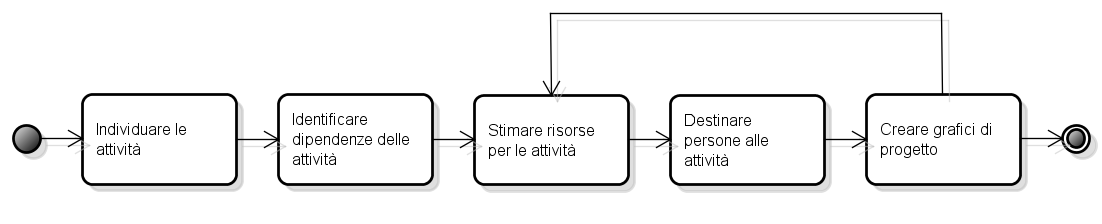
\includegraphics[scale=0.50]{../modello/img/pianificazione.png}}
        \end{picture}
\begin{center}
Diagramma di attivit\'a per la pianificazione di progetto.
\end{center}
L' attivit\'a di identificazione delle dipendenze necessita di particolare attenzione in quanto \'e necessario che vengano identificati i cammini critici, cio\'e quelle sequenze di attivit\'a con dipendenze funzionali critiche e dipendenze temporali strette. Ogni attivit\'a \textbf{critica} dovr\'a quindi essere classificata come tale nel caso in cui un suo ritardo crei un esffetto di rallentamento o in generale dannoso per lo svolgimento di altre attivit\'a~. Tali attivit\'a nella rappresentazione con il diagramma di Gantt verranno differenziate da quelle \textbf{non critiche} con il colore rosso.
\subsubsection{Analisi}
Questo periodo si \'e esteso per 28 giorni, dal \textit{2014-02-05} al \textit{2014-03-05} ed i ruoli che sono stati maggiormente coinvolti sono: \textit{Responsabile}, \textit{Amministratore} e \textit{Analista}.
In questo periodo si \'e cercato di lavorare a stretto contatto per instaurare un rapporto di fiducia tra i membri del \textit{team} creando un ambiente di fiducia comunicando apertamente.
\\
Il gruppo \gruppo ha lavorato per poter presentare i seguenti documenti alla consegna del \textit{2014-03-05}:
\begin{itemize}
	\item \textbf{Norme di progetto:} documento che dovrebbe essere redatto a "tempo zero", viene steso dall' \textit{amministratore} e fissa regole, procedure e strumenti funzionali al raggiungimento degli obbiettivi strategici. Tale documento \'e stato steso prima di ogni altro in quanto vincola le modalit\'a di stesura, e non solo, di tutti gli altri documenti che dovranno essere prodotti. Per questo motivo le attivit\'a ad esso correlate saranno critiche.
	\\ Il rispetto di tali norme verr\'a attestato dai verificatori;
	\item \textbf{Studio di Fattibilit\'a~:} l' \textit{analista} designato valuta i vari capitolati d' appalto forniti e ne analizza vari fattori: complessit\'a~, vantaggi, svantaggi e interesse nel suo svolgimento. Le attivit\'a del processo di stesura di questo documento sono critiche in quanto senza di esso non si pu\'o procedere con l' analisi dei requisiti;
	\item \textbf{Analisi dei requisiti:} L' attivit\'a di stesura di questo documento ha termine solo se il documento supera con successo la revisione di progettazione. Durante il periodo di analisi si cercher\'a di identificare al meglio i requisiti del sistema;
	\item \textbf{Piano di progetto:} Il \textit{Responsabile} per mezzo di questo documento fissa le risorse disponibili, la suddivisione delle attivit\'a ed il calendario ad esse connesso; 
	\item \textbf{Piano di qualifica:} Questo documento fissa le strategie di verifica del gruppo e viene redatto dall' \textit{Analista} con la stretta collaborazione del \textit{Responsabile} e dell' \textit{Amministratore} per la sua buona stesura;
	\item \textbf{Glossario:} Scritto e mantenuto costantemente aggiornato dai membri del gruppo contenente termini ambigui o poco chiari, necessari per la corretta interpretazione dei documenti;
	\item \textbf{Lettera di presentazione:} Documento necessario per permettere al gruppo di partecipare alla gara d' appalto, il destinatario \'e il committente.
\end{itemize}
 \setlength{\unitlength}{1mm}\begin{picture}(0,70)
                \put(0,0){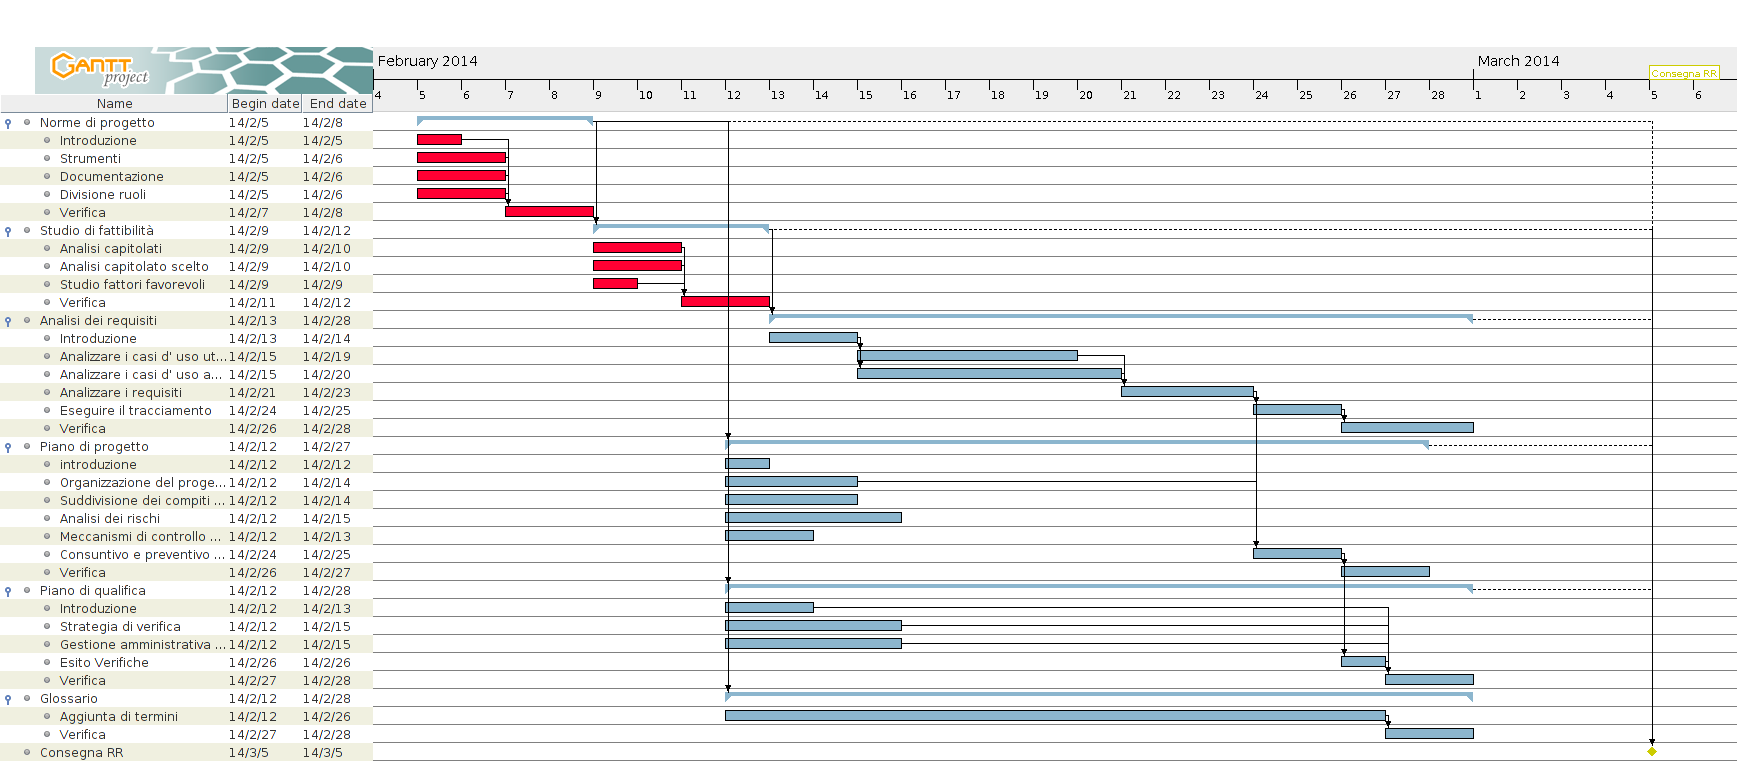
\includegraphics[scale=0.25]{../modello/img/RR.png}}
        \end{picture}
\begin{center}
Immagine 1: Diagramma di Gantt, periodo di Analisi
\end{center}
\subsubsection{Progettazione Architetturale}
Questo periodo si \'e esteso per 18 giorni, dal \textit{2014/03/11} al \textit{2014/03/29} ed i ruoli che saranno maggiormente attivi saranno: \textit{Responsabile}, \textit{Amministratore}, \textit{Progettista}, \textit{Verificatore} e \textit{Analista}. Nel primo intervallo di questo periodo il team andr\'a a correggere gli errori segnalati all' uscita dalla \textbf{RR}\ped{G} ponendo particolare attenzione all' analisi dei requisiti in quanto sar\'a con molta probabilit\'a da correggere e necessiter\'a di incremento; solo successivamente si potr\'a andare a incrementare i documenti gi\'a esistenti e a stendere la \textbf{Specifica  Tecnica}. Tale documento, redatto dal \textit{Progettista}, conterr\'a una modellazione del sistema \textit{Software} con una prima caratterizzazione architetturale dei componenti.\\
 \setlength{\unitlength}{1mm}\begin{picture}(0,72)
                \put(0,0){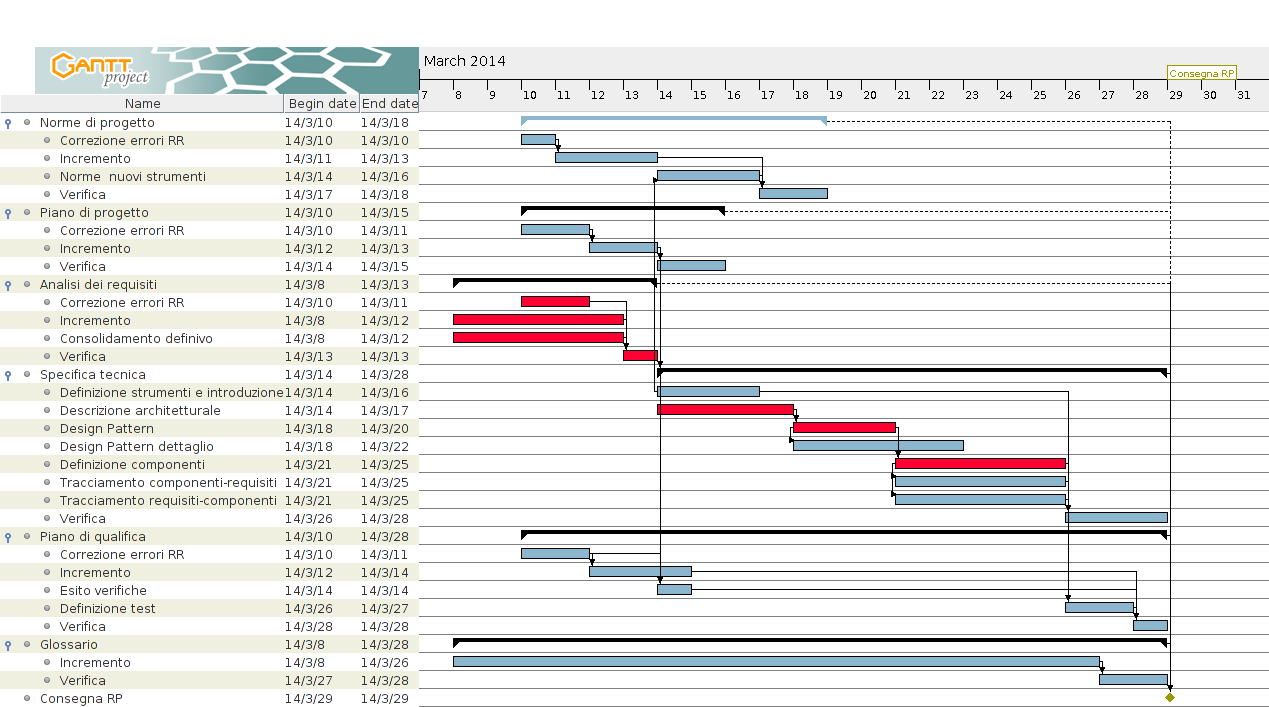
\includegraphics[scale=0.30]{../modello/img/RP.png}}
        \end{picture}
\begin{center}
Immagine 2: Diagramma di Gantt, periodo di Progettazione Architetturale
\end{center}
\subsubsection{Progettazione di Dettaglio e Codifica}
Periodo che si estende dal \textit{2014-04-14} al \textit{2014-06-28}. Durante questo lasso di tempo i ruoli maggiormente coinvolti saranno: \textit{Progettista}, \textit{Programmatore} e \textit{Verificatore}. I documenti prodotti in questo periodo saranno:
\begin{itemize}
	\item \textbf{Definizione di Prodotto}: Definisce nel dettaglio la struttura del sistema per fornire una struttura dettagliata che verr\'a poi utilizzata dai \textit{programmatori} per la codifica. I suoi contenuti si baseranno su quanto presente nella \textit{Specifica Tecnica};
	\item \textbf{Manuali utente} Questi documenti saranno utilizzati dagli utenti del sistema per ottenere informazioni sull' utilizzo del \progetto~.
\end{itemize}
Dovranno essere inoltre essere eseguite le seguenti attivit\'a~:
\begin{itemize}
\item \textbf{Codifica:} i programmatori basandosi su quanto riportato nella \textit{Definizione di Prodotto} forniranno una versione del sistema funzionante;
\item \textbf{Test} Si eseguiranno i test pianificati e si analizzeranno i risultati ottenuti.
\end{itemize}
 \setlength{\unitlength}{1mm}\begin{picture}(0,46)
                \put(10,0){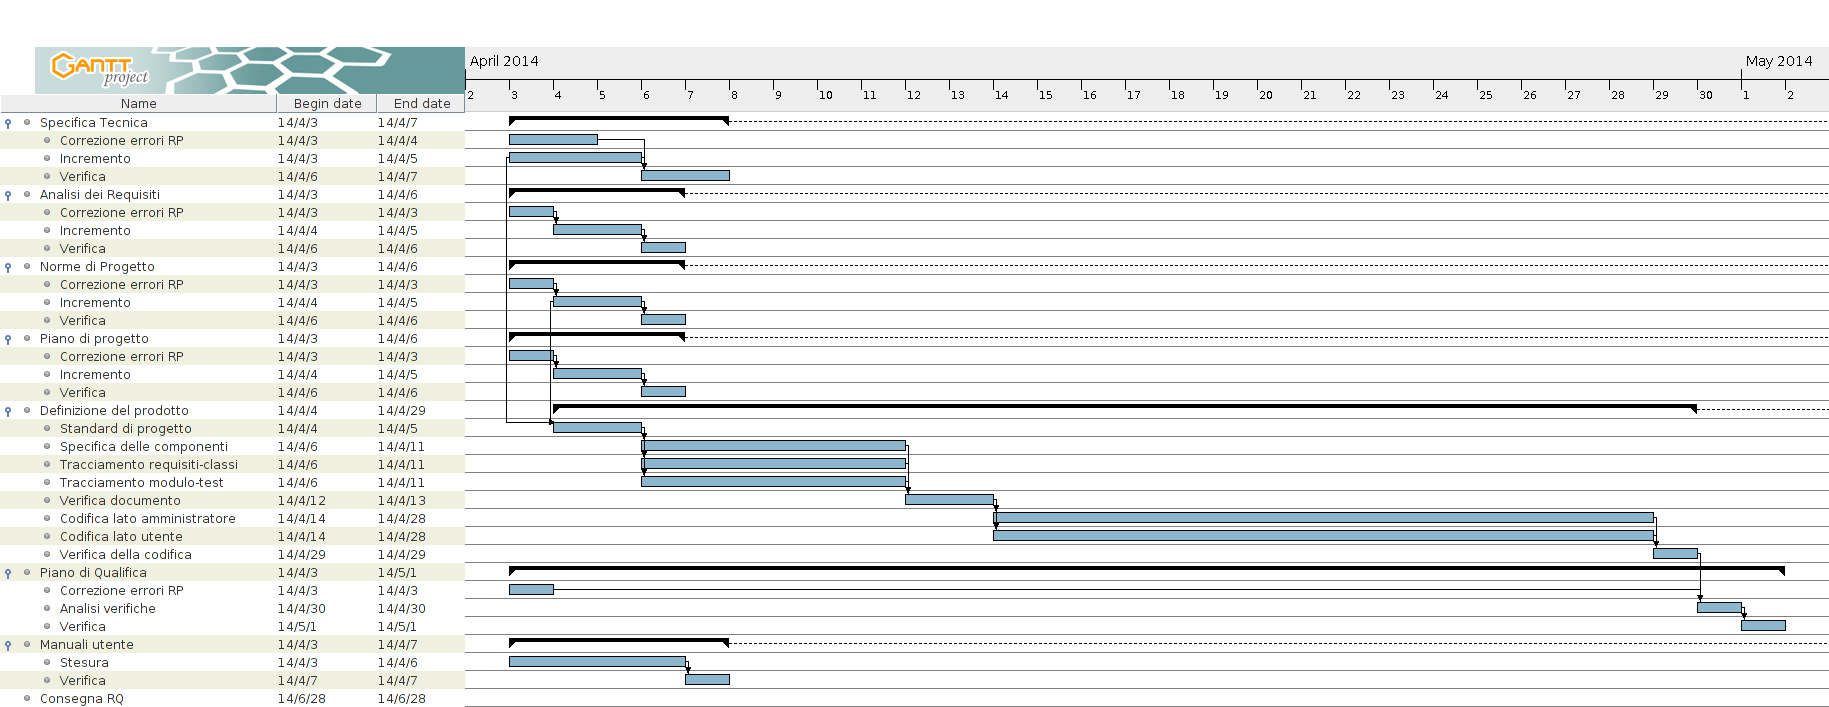
\includegraphics[scale=0.19]{../modello/img/RQ.png}}
        \end{picture}
        \begin{center}
Immagine 3: Diagramma di Gantt, periodo di Progettazione di Dettaglio e Codifica
\end{center}
\subsubsection{Verifica e Validazione}
Dal \textit{2014-07-03}  \textit{2014-07-18} il gruppo lavorer\'a per terminare il processo di sviluppo del \textit{software}. In questo periodo si dovranno eseguire le seguenti attivit\'a~:
\begin{itemize}
	\item \textbf{Incremento e verifica finali: } I documenti riceveranno le ultime modifiche e poi dovranno essere verificati e validati;
	\item \textbf{Codifica:} In base alle ultime modifiche effettuate alla \textit{Definizione di Prodotto} si dovr\'a produrre la versione corrispondente del sistema e verificarne la correttezza;
	\item \textbf{Test e collaudo:} Si effettueranno gli ultimi test sul sistema per assicurarsi il suo corretto funzionamento e il collaudo generale, testandone le funzionalit\'a.
\end{itemize}
 \setlength{\unitlength}{1mm}\begin{picture}(0,87)
                \put(0,0){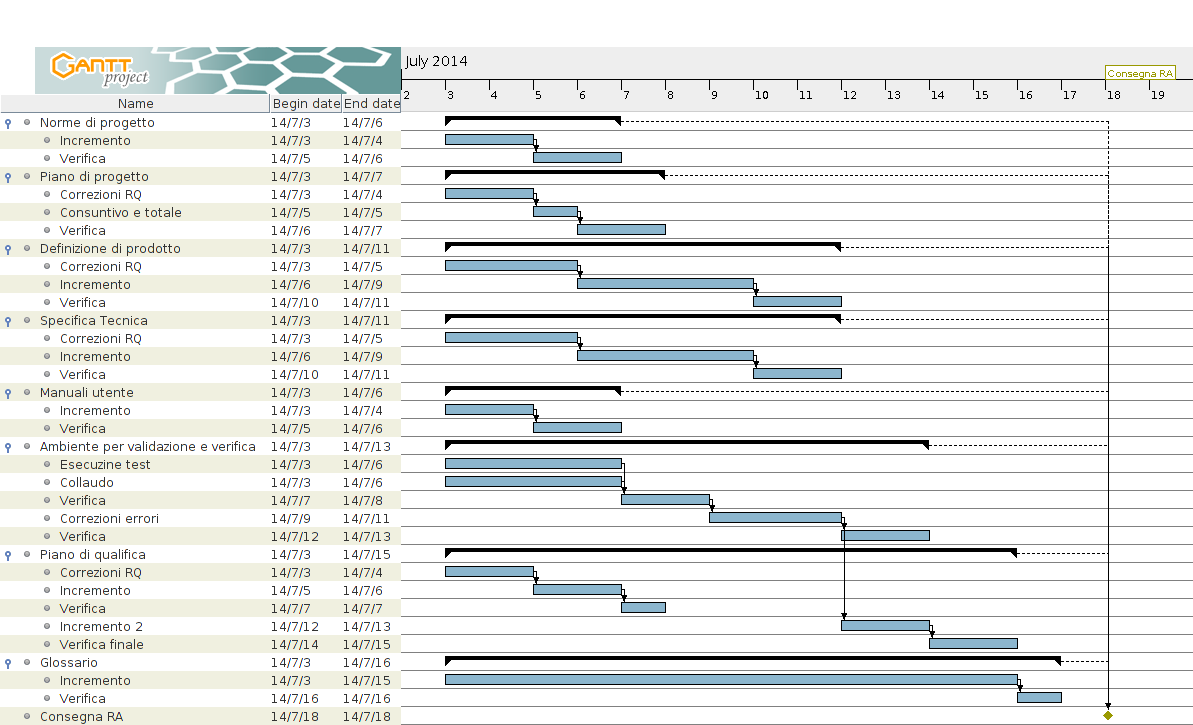
\includegraphics[scale=0.35]{../modello/img/RA.png}}
        \end{picture}
        \begin{center}
Immagine 4: Diagramma di Gantt, periodo di Verifica e Validazione
\end{center}